\documentclass[conference]{IEEEtran}
\IEEEoverridecommandlockouts
% The preceding line is only needed to identify funding in the first footnote. If that is unneeded, please comment it out.
\usepackage{cite}
\usepackage{amsmath,amssymb,amsfonts}
\usepackage{algorithmic}
\usepackage{graphicx}
\usepackage{textcomp}
\usepackage{stmaryrd}
\usepackage{verbatim}
\usepackage[]{mdframed}
\usepackage{setspace}
\usepackage{caption}
\usepackage{hyperref}
\setstretch{1.5}
\newcommand{\BibTeX}{\textrm{B \kern -.05em \textsc{i \kern -.025em b} \kern -.08em
T \kern -.1667em \lower .7ex \hbox{E} \kern -.125emX}}
\begin{document}

\title{Symmetric Encryption of Audio \\ via Chaotic Neural Networks}

\author{\IEEEauthorblockN{1\textsuperscript{st} Patrick Pfenning}
\IEEEauthorblockA{\textit{School of Computing and Data Science} \\
\textit{Wentworth Institute of Technology}\\
Boston, MA \\
pfenningp@wit.edu}
}

\maketitle

\begin{abstract}
This paper focuses on developing a new algorithm for encrypting audio files symmetrically using a Chaotic Neural Network (CNN).
Central to our methodology is an iterative application of chaotic maps, where each hidden layer of the network represents a different chaotic attractor.
This process engenders the generation of a pseudo-random arrays which are reduced to a singular cipher array, our encryption key.
Said cipher is applied to the bitmap for each channel of the supplied Wave Audio File (WAV), and thus creating a secure ciphertext.
A comprehensive assessment is conducted to benchmark the efficacy of our approach, evaluating both computational efficiency and strength of encryption.
These findings include: an average increase in entropy rate of $2.02$, a peak signal-to-noise ratio of $4.09$, nearly identical to that of a random array, and a correlation to plaintext of $1.40\times10^{-5}$, an order of magnitude less than a random input.
This study not only represents a novel encryption algorithm for audio, but contributes to a larger discussion of the importance of security and encryption in our increasingly technological world.
\end{abstract}

\begin{IEEEkeywords}
chaos, encryption, audio, neural networks, pseudo-random, symmetric-key, lorenz, logistic, henon, ikeda
\end{IEEEkeywords}

\section{Introduction}\label{sec:introduction}
The world we live in has become wildly dependent on the fast transfer of information.
Everything, from our work and education to our entertainment and social life, often requires the internet as a medium.
With this abundance of information, how can one ensure that their personal data remains private to bad actors?
Enter the field of encryption, the process of encoding information.
Encryption allows one to take a plaintext message we wish to transmit and transform it into a ciphertext.
This ciphertext is illegible to those who do not have a \textit{key}.

Most modern encryption processes create a \textit{psuedo-random} key via a defined algorithm.
These algorithms can be broken into two schemes: \textbf{Symmetric-key Encryption} and \textbf{Public-key Encryption.}
Symmetric-key Encryption algorithms create a single secret key which both the sender and receiver have.
This key is used to both encrypt and decrypt the message.
The security of this method directly depends on the holders of the key as anyone who has it can read the cipher.
Public-key Encryption algorithms require the message receiver to generate both a public and private key.
The receiver shares the public key with the trusted sender who uses it to encrypt a message.
The message is sent to the receiver where the private key is used to decrypt it.
Because the private key is the only way to decipher the message, public-keys can be shared with impunity.
Though both methods do nothing to prevent the cipher from being intercepted by a third party, if the algorithm is strong enough, it should be illegible.

Billions of packets of information flow throughout the internet on a daily basis.
The larger the packet, the longer the encryption will take.
In this paper, we will develop our own algorithm to encrypt several audio files of varying sizes.
The aforementioned algorithm will be developed using what is known as a \textbf{Chaotic Neural Network} (CNN).
This algorithm will be symmetric similar to \textbf{Advanced Encryption Standard} (AES).

\section{Literature Review}\label{sec:literature-review}
\subsection{\textbf{Chaos: An Introduction to Dynamical Systems}~\cite{Alligood}}\label{subsec:chaos:-an-introduction-to-dynamical-systems}

Alligood provides an excellent course in the study of such dynamical systems.
She successfully explains chaotic phenomena in nature using Linear Algebra, Differential Equations and Numeric Analysis.
The book defines chaos as a field of study while introducing the idea of chaotic maps.
These maps are recursive in nature, and are highly sensitive to initial conditions.
Each iteration is mapped to a new phase-space for which the rate of separation of points in the sequence is directly related to the system's Lyapunov Exponents.
There is one exponent for each degree of freedom the chosen system has.
The scalar value of the exponent determines how the basis stretch ($LE > 1$) or shrink ($LE < 1$).
Sequences created by such maps, though deterministic, can be unstable.
These unstable sequences are known as chaotic orbits.
This instability is statistically indistinguishable in nature to randomness, making them ideal candidates for providinging repeatable pseudo-random arrays.

\subsection{\textbf{A Review on Applications of Chaotic Maps in Pseudo-Random Number Generators and Encryption}~\cite{Naik2022}}\label{subsec:a-review-on-applications-of-chaotic-maps-in-pseudo-random-number-generators-and-encryption}

In 2019 Naik and Singh gave a detailed review of Chaotic Neural Networks applications for encryption.
The key aspect, as in many of the papers in this section is the creation of a viable generator.
One way chaotic maps are used to generate a sequence of length \textbf{N}, which is equal to the byte-length of the plaintext file.
These values are then converted to binary and one byte are taken from each value, often the first byte after the decimal point.
This sequence is then reshaped to match the dimensions of the file being encrypted.
The resulting matrices are then XORed with the original file masking the data.
If we preform this action a second time, we will revert to the original data.
This is extremely useful for the decryption process.

This paper also goes through another chaotic tool, diffusion, the act of swapping indices.
The Arnold Cat Map (ACM)~\cite{Naik2022} provides an efficient way to diffuse desired file prior to encrypting, but is most often used for image encryption only.
After several iterations of this map on a matrix the original data is unrecognizable.
It should be noted that orbits of ACM are finite, therefore if the map is iterated to the length of the orbit, all diffusion will be undone.

The largest takeaway of this paper is the review of an audio encryption model using sequences from the Henon and Tent maps.
Said sequences are XORed to create a secret key.
This secret key is then XORed with the audio file to encrypt.
Their correlation coefficient between the plain and ciphered files were as low as 0.0014 with entropy was as high as 7.9995.

\subsection{\textbf{Comparison of Cryptography by Chaotic Neural Network and by AES}\cite{Skovajsova2019}}\label{subsec:comparison-of-cryptography-by-chaotic-neural-network-and-by-aes}

This 2019 paper by Skovajsová~ gives a step by step explanation of how AES encryption works and compares it to a prebuilt CNN\@.
Both algorithms were tested on five random images of each of the following sizes: 512b, 1024b, 2048b, 3KB, 30KB and 3MB\@.
For both ciphering and deciphering, the CNN significantly outperformed the AES model in terms of speed.
The ciphertext created by both models were identical in size to the plaintext file, showing no degradation of information.
It was noted that the CNN used here was a Hopfield network that 1D chaotic maps for its neural weights.
1D maps are much faster for generation, but only require a single initial value.
If this initial condition is found by a bad actor, the algorithm will be broken.
To counteract this, we will be building multiple layer networks of varying dimensionality, each requiring unique sets initial conditions.

\section{Methodology}\label{sec:methodology}

\subsection{Generalization}\label{subsec:generalization}

Suppose there exists some audio file $A$ which we wish to encrypt with our cipher\@.
We first transform $A \rightarrow A^\prime$, such that $A^\prime$ is the matrix containing the header bytes of $A$~\cite{app112110190}.
We now define $N$ to be byte length of $A^\prime$.

We now supply $N$ as a global parameter of our network.
Networks layers are a chosen chaotic map with a unique initial conditions corresponding to:

\begin{mdframed}
\begin{enumerate}
    \item The chosen parameters of the map.
    \item Input variable for each dimension of the map.
    \item Some integer $k$ defining the number of iterations to remove from the generator.
    \item The byte-length $N$, the desired length of our cipher.
\end{enumerate}
\end{mdframed}

For each layer $i$ we plug in our parameters, supply our input variables and iterate the map $k_i+N$ times.
This results in set of a matrices $Z_{d_i \times (k_i+N)}$ such that $d_i$ is the of dimensionality of our chosen maps, and $k_i$ is said map's primer.
Similar to steps in other papers~\cite{Lokesh,app112110190}, we reduce our matrices using the following transformation:

\begin{equation}\label{eq:bitmap}
    W = \bigoplus^{i} \bigoplus^{j} \big\lfloor  Z_{(i, j, k_i:N)} \times 10^{\frac{b}{2}} \big\rfloor \mod 2^{b}
\end{equation}

Such that $i$ denotes a hidden layer of our network, $j$ represents a dimension of the layer's map.
We use the $k_i:N$ to state that we will only take the last $N$ iterations of each matrix.
$W$ is the logical XOR to the byte-wise representation of our chaotic outputs, resulting in an array of length ${N}$.

$W$ can now be used to find our ciphertext such that $E^\prime=A^\prime \oplus C$.
When the sample rate of $A$ is applied to $E^\prime$, it becomes the encrypted audio file $E$.
Given the properties of the XOR operation, $C$ acts as both our encryption and decryption such that:

\begin{equation}\label{eq:xored}
    A^\prime = A^\prime \oplus W \oplus W = E^\prime \oplus W = A^\prime
\end{equation}

This satisfies the requirements of symmetric key encryption.
Theoretically, this methodology should work for any set of chaotic maps we choose.
Because chaotic maps are psuedo-random in nature, the same map can be used in multiple layers, provided that at least one of the map's parameters and/or input variables differ.
It is important to state that because of how $W$~\eqref{eq:bitmap} is calculated, if two layers are identical they will cancel each other out.
Through the rest of this paper we will develop an algorithm using this methodology with our chosen set of chaotic maps.

\begin{mdframed}
\textbf{NOTE:} It is possible for $A$ may have multiple channels of audio.
In cases such as this, we apply $C$ to each channel individually.
This may also open the door to image encryption in the future.
\end{mdframed}

\subsection{Choosing Our Maps}\label{subsec:choosing-our-maps}

We have chosen audio as our medium for encryption.
For ease of use, we will be using Waveform Audio File Format.
Byte representations of these files can be interpreted as $8$-bit or $16$-bit integers thus fitting our methodology nicely.
We have chosen to develop a network consisting of four hidden layers, each representing their own map.
The first layer we will use is the two-dimensional Hénon Map~\cite{Hamdy}:

\begin{equation}\label{eq:Henon}
\begin{aligned}
    x_{n+1} &= 1 - ax_n^2 + y_n \\
    y_{n+1} &= bx_n
\end{aligned}
\end{equation}

\noindent Chaotic behavior occurs here with parameters $a=0.3$ and $b=1.4$.

Our second layer will also be two-dimensional, the Ikeda Map~\cite{app112110190} :

\begin{equation}\label{eq:Ikeda}
\begin{aligned}
    x_{n+1} &= 1 + u(x_n \cos(t_n) - y_n \sin(t_n))\\
    y_{n+1} &= u(x_n \sin(t_n) + y_n \cos(t_n))\\
    t_{n+1} &= \beta - \frac{\gamma}{1+x_{n+1}^2+y_{n+1}^2}
\end{aligned}
\end{equation}


\noindent Where this system develops a chaotic attractor whenever $u\ge0.6$.

Adding complexity, we turn to the three-dimensional map known as the Lorenz attractor~\cite{Naik2022}.

\begin{equation}\label{eq:Lorenz}
\begin{aligned}
    \dot{x} &= \sigma (y - x)\\
    \dot{y} &= x (\rho - z) - y\\
    \dot{z} &= xy - \beta z
\end{aligned}
\end{equation}

\noindent We will use parameter values $\sigma=10$, $\beta=\frac{8}{3}$ and $\rho=28$.
This map is most famous for \textit{The Butterfly Effect}~\cite{Alligood}, and is commonly used in weather prediction.

Finally, we introduce the Logistic Map~\cite{Qin2017}:

\begin{equation}\label{eq:Logistic}
    x_{n+1} = r x_n (1 - x_n)
\end{equation}

\noindent Such that $r=4$.
It should be noted that $x_0 \in [0,1]$ for chaotic behavior to occur.

Due to the transitive properties of XOR shown in ~\eqref{eq:xored}, the order of these layers is of no consequence.
In fact, these maps will be calculated in parallel, and then be reduced to $W$~\eqref{eq:bitmap}.

\section{Key Generation}\label{subsec:key-generation}

To create our key we simply follow the steps laid out in Section \ref{sec:methodology}, and do the following:

\begin{enumerate}
    \item Choose our maps. Remember that order has no impact.
    \item Set our parameters for the map. It should be noted that not all parameters lead to chaotic attractors, so please choose known chaotic parameters like those given in Section \ref{subsec:choosing-our-maps}.
    \item Choose initial conditions. A random value in the range $[0, 1]$ often suffices.
    \item Set a primer. This gives us some separation from our initial conditions.
\end{enumerate}

\noindent The table below provides an example key using the aforementioned steps:

\begin{tabular}{llll}
    \hline
    \textbf{map} & \textbf{parameters} & \textbf{primer} & \textbf{initial condition} \\
    \hline
    henon & [1.4, 0.3] & 171 & [0.055, 0.005]\\
    ikeda & [0.9] & 353 & [0.068, 0.377]\\
    logistic & [4] & 250 & [0.945]\\
    lorenz & [10, 28, 2.67] & 817 & [0.459, 0.137, 0.726]\\
    \hline
\end{tabular}
\\

This key can now be used as input for our hidden layers, with outputs being reduced to our cipher $W$.

\section{Experimentation and Results}\label{sec:experimentation-and-results}

\subsection{Processing Time and Complexity}\label{subsec:processing-time-and-complexity}

One major fault of this process is efficiency.
As this method is in its infancy, it has yet to be optimized like AES and RSA\@.
Though efforts were made to optimize code using modules like \textit{numpy} and \textit{numba}, python itself is slow.
The below image shows a Log-Log graph of encryption time vs file size:

\begin{center}
    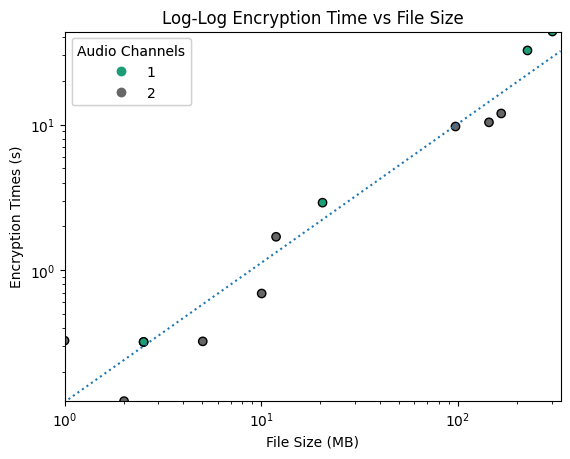
\includegraphics[scale=.5]{images/loglog}
\end{center}

We see that this image shows this algorithm may be $O(n^2)$, taking exponential time to encrypt as file size increases.
Currently, each cipher is recreated in full each run.
Because all sequences used are chaotic deterministic, methods like hash tables could be of use in the future.
The only input for our cipher is byte-length, so if we have encrypted a file of length N, we can also encrypt files smaller than N\@.

\subsection{Entropy Analysis}\label{subsec:entropy-analysis}

Shannon Entropy measures the uncertainty of a value given random choice.
We used this metric to show the randomness of values within an array.
All matrices used in this section, as well as the two following, have only integer values in the range $[-2^{16}, 2^{16}]$.
Audio files generally have a high entropy as they are often one dimensional and time variant.
Thus, the goal here is to have a significant increase in entropy from plaintext to comparison.
In this experiment we found entropy for plaintext audio, the encrypted audio and a random array of the same shape.

\begin{tabular}{|l|l|}
    \hline
    \textbf{Entropy of Plaintext Audio} & 9.015836 \\
    \textbf{Entropy of Encrypted Audio} & 11.038566 \\
    \textbf{Entropy of Random Array} & 11.674987 \\
    \hline
\end{tabular}
\\

As stated above, audio has a high level of entropy as compared to static arrays like images.
This is because surrounding pixels are associated by position rather than time.
The baseline entropy we received from our plaintext was just over 9.
In comparison, both the encrypted and random arrays showed an increase to 11, denoting a higher level of variance in choice than the plaintext.
With entropy, as well as the following metrics, we hope to find that our encrypted metric is comparable to that of the random array.


\subsection{Peak Signal to Noise Ratio}\label{subsec:peak-signal-to-noise-ratio}

The Peak Signal to Noise Ratio (PSNR) measures similarity between two images.
This process is often used to determine loss of quality when compressing an image.
Outcomes are measured on a percentage scale, with 100 stating the images being compared are identical.
For our intents and purposes, we hope to minimize our PSNR value.
Because we are using audio files, we converted our arrays to an image.
To do this, we took the absolute value of our array, divide by the maximum, and multiply by 255.
This results in an array of floats from 0 to 255, which can then be read as an image.
The below table gives the PSNR for our plain audio verses the encrypted file, the decrypted file and a random array of the same dimensions.

\begin{tabular}{|l|l|}
    \hline
    \textbf{PSNR of Encrypted Audio} & 4.094938 \\
    \textbf{PSNR of Decrypted Audio} & 100.000000 \\
    \textbf{PSNR of Random Array} & 4.093613 \\
    \hline
\end{tabular}
\\

We expect our decrypted file to be equivalent to the plaintext.
With a PSNR of 100, that expectation is verified.
We now notice that the encrypted file and the random array have nearly identical PSNR.
Not only does our encrypted file extremely dissimilar from its plaintext counterpart, it is almost indistinguishable from that of a random sequence.

\subsection{Correlation Analysis}\label{subsec:correlation-analysis}

Another direct comparison between files is correlation.
This metric was taken at the channel level, therefore each array in stereo WAV file is considered to be its own object.
To do this created a matrix with two columns, the first always the plain audio channel, with the second as the desired comparison array.
We again checked three cases, encrypted, decrypted and random.
Correlation provides outputs in the range $[-1, 1]$, with $1$ being perfect positive correlation, and $-1$ as perfect negative.
We want no correlation between the encrypted and plain file, and thus are looking for a correlation close to zero.

\begin{tabular}{|l|l|}
    \hline
    \textbf{Encrypted Audio vs Plain Audio} & 0.000014 \\
    \textbf{Decrypted Audio vs Plain Audio} & 1.000000 \\
    \textbf{Random Array vs Plain Audio} & 0.000233 \\
    \hline
\end{tabular}
\\

As a sanity-check, we see that out decrypted file has a perfect positive correlation with the plaintext, as intended.
Encrypted files showed an extremely low correlation, $1.40\times10^{-5}$, which is an order of magnitude smaller than that of random arrays.
Therefore, we have shown that our encrypted file shows no correlation with its plaintext counterpart.


\subsection{Key Sensitivity}\label{subsec:key-sensitivity}

Given the nature of chaotic sequences, and set of unique initial conditions will never overlap.
Chaotic sequences exist in a fractional dimension, and can fill the space with the next integer dimension above it.
These sequences can hit all real points within a dimension without having any volume in said space.
For example, The Lorenz Attractor~\cite{Alligood} has a fractional dimension just over two, but can fill a three-dimensional space.
This behavior contributes to chaotic sensitivity to initial conditions.
The below figure shows examples for each of our four chaotic maps with two unique keys.
Points of these sequences will never overlap, and thus are highly reactive to any change.
Unless a bad actor knows the exact values chosen for a key, they will be unable to decipher the encrypted message.
Keys are highly sensitive to change to any parameter, initial condition or primer.

\begin{center}
    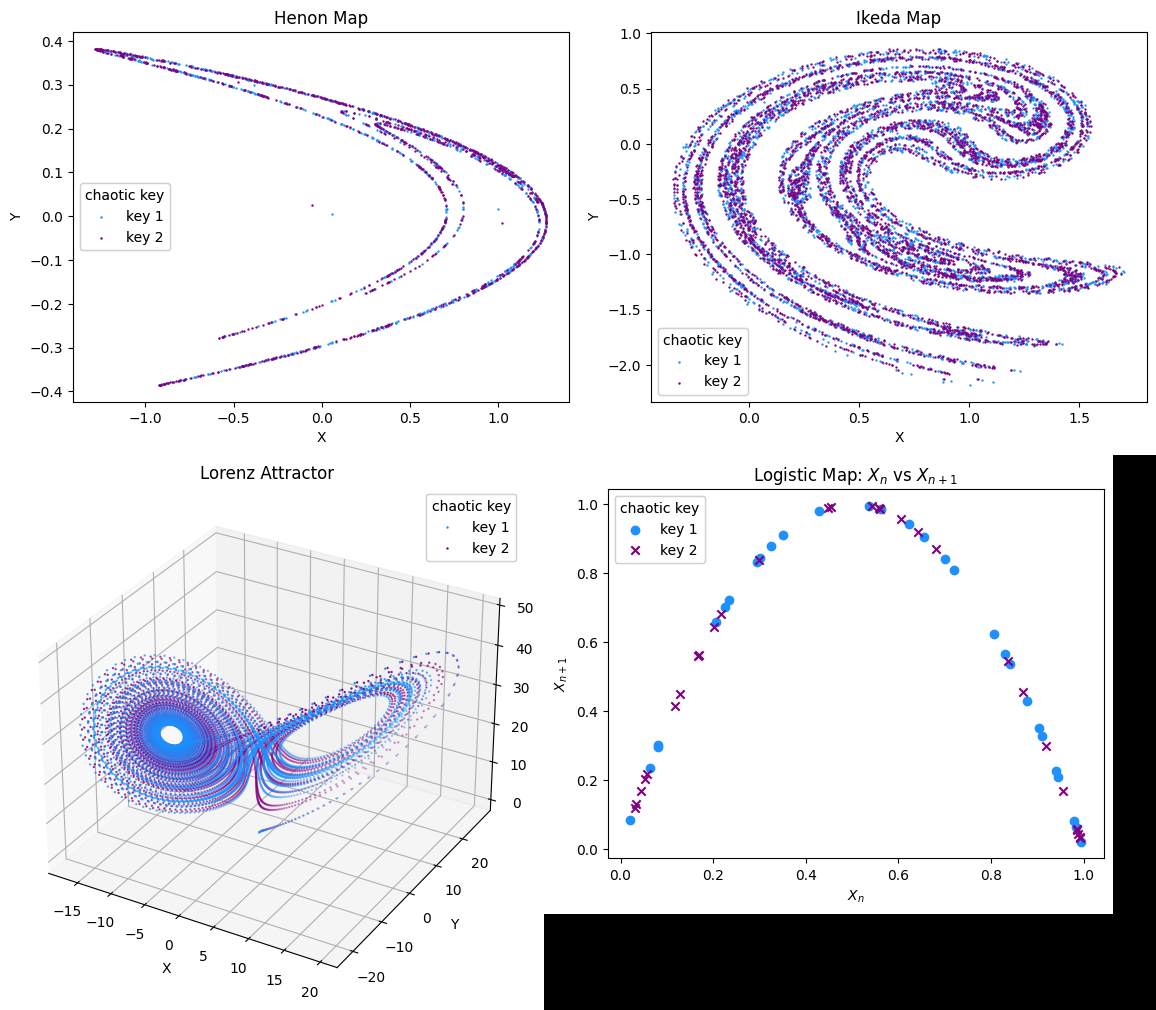
\includegraphics[scale=.2]{images/KeySen}
\end{center}


\section{Future Work}\label{sec:future-work}

This process need not be limited to audio encryption.
Given that we are just creating a cipher from a given byte length, this application may be applied to any binary array.
This includes, but is not limited to: text, other audio mediums, image, and video.
We intend to maintain the code associated with this project which can be found in the following repository \href{https://github.com/ppfenning/Symmetric-Encryption-via-CNN}{\textbf{Symmetric-Encryption-via-CNN}}.
We hope to add more chaotic options, as well as a text interface to choose the key order, including multiple instances of the same map within a key.

\section{Conclusion}\label{sec:conclusion}

In terms of theory, we have shown that encryption via chaotic sequences is both repeatable and effective.
In order to be practical, efficiency of this process must be addressed.
Given the high level of key sensitivity, as well as the variablity of map choice, keys such as this will be immensely difficult to crack.
Future work, include direct comparison to existing methodologies, are still on the horizon.
We do however believe this process shows immense promise in the field of encryption.

\bibliographystyle{ieeetr}
\bibliography{bib/bibliography}

\end{document}
